\chapter{Event reconstruction}\label{chap:reconstruction}

%\chapterquote{}{}

\section{Introduction}

The reconstruction and identification of particles with the \CMS detector starts from the hits of ionising particles and energy deposits of particles showers. The granularity of the \CMS detector allows muons, electron and photons, and charged and neutral hadrons to be distinguished. Instead of simply detecting, reconstructing and identifying particles with their respective dedicated system, information from all aspects of the detector are correlated to extract the best estimate for the reconstructed set of particles. Each particle is distinguish individually by a technique known as particle flow (PF).

The initial step in reconstruction, prior to the PF method, consists of forming charged particle tracks from hits in the silicon tracker, tracks in the muon chambers and calorimeter clusters from energy deposits in the calorimetry system. The basic building blocks form the input into the PF algorithm which attempts to link the various blocks into a coherent picture of a particle candidate. For example, tracks are linked to an \ECAL deposit to form an electron candidate. These are further linked to \ECAL deposits consistent with Bremsstrahlung photons from the original electron track. These secondary photons may undergo further interactions resulting in displaced electrons tracks also linked to the primary electron. Furthermore, the reconstruction of all particles results in a simple \ptmiss calculation from the negative vector sum of all particle momenta.

This chapter will describe in detail the process of tracking, clustering and the PF method in the full reconstruction of a proton-proton interaction.


\section{Tracking}

Charged particles originating from the interaction point travel outward through the magnetic field in helical trajectories. The hits in the silicon tracker are reconstructed into the track by a fitting procedure known as the combinatorial track finder. Hits are formed within the pixel tracker by clustering deposits, above a certain threshold, in adjacent pixels. The position of the hit for single pixel clusters is taken at the centre of the pixel while multi-pixel clusters have a charge-weighted position, correcting for the drift of electrons in the magnetic field. A more sophisticated, albeit, computationally demanding method is used for the final track fit which involves a $\chi^2$-fit of expected charge deposits from a large number of simulated particles through the pixels to the observed charge deposit, accounting for pixel deterioration. Strip tracker hits are formed from clusters of adjacent strips with charge deposits exceeding a noise-level. The hit position is determined from a charge-weighted average of the cluster, correcting for the electron drift in the magnetic field and known inefficiencies with the charge collection. All hits have an associated uncertainty propagated to the track fitting procedure~\cite{Chatrchyan:1704291}.

The combinatorial track finder involves a series of Kalman filters (KF) \cite{Kalman:1960} --- a recursive parameter estimator. A Kalman filter starts with an initial state (a seed), typically from a guess or estimation, and iterates across measurements updating the initial state parameters by comparing the prediction to the observations. For track fitting, the fit is performed to five parameters which describe points along a helical track, known as the perigee parameterisation:
%
\begin{equation}
    \left( \frac{q}{\pt}, x_t, y_t, \theta_t, \phi_t \right)\ \,
\end{equation}
%
where $q/\pt$ is the ratio of the charge to track transverse momentum to give the signed curvature scale of the trajectory. The parameters $x_t$ and $y_t$ are the distances from the interaction point to a point along the trajectory in the $\vec{x}_t$ and $\vec{y}_t$ axis, shown in Fig.~\ref{fig:kf_parameters} along with the definitions of the angles $\theta_t$ and $\phi_t$.

\begin{figure}
    \centering
    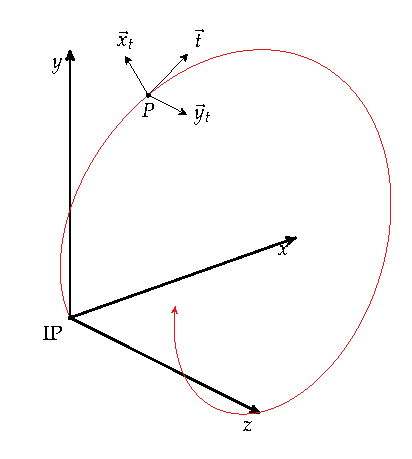
\includegraphics{diagrams/tikz/kf_parameters/kf_parameters.pdf}
    \caption[Coordinate system to describe the curved path of a charged particle within an magnetic field.]{
        Diagram of a track (shown in red) from the interaction point (IP) with the conventional \CMS coordinate system as well as a local coordinate system along the trajectory, an example of which is shown at point $P$ where $\vec{t}$ is the tangential vector, $\vec{x}_{t}$ is perpendicular to both the z-axis and $\vec{t}$ and $\vec{y}_{t}$ is the remaining vector to create a right-handed coordinate system. The angle between the $x$-axis and the projection of ${\vec{t}}$ onto the $x$-$y$ plane is $\phi_t$. Similarly, the angle between the $y$-axis and the projection of ${\vec{t}}$ onto the $y$-$z$ plane is $\theta_t$.
    }
    \label{fig:kf_parameters}
\end{figure}

The trajectory building with a Kalman filter starts with the seed generation stage by combining a set of pixel hits, where the resolution is the greatest and occupancy the lowest. Each iteration of the Kalman filter extends to the next tracker layer where each hit candidate, within a $\chi^2$ window, is kept to form independent track candidates. Fake tracks will typically have a layer where no hits are within the window and can be dropped. Further checks are performed on the consistency of hits with the \pt of the track, in addition to vertex constraints. Finally, a cleaning process assigns unique tracks to a seed and vice versa. After determining the full set of tracks, the Kalman filter procedure is repeated with the precise hit reconstruction, accounting for inter-layer material and field inhomogeneities, with inflated uncertainties to avoid biasing the initial result. Furthermore, the Kalman filter is repeated, seeded by hits from the outermost layer iterating inwards.  The best fit tracks are taken from an average of the Kalman filter starting from the inner layers and the reverse.

The trajectory building is performed ten times with different seeds to target various classes of tracks with hits associated with candidate tracks removed from subsequent iterations:
\begin{itemize}
    \item Prompt and high \pt tracks, and $b$-hadron decays are targeted by the first three iterations, seeded by three hits in the pixel detector with constraints on the track \pt and distance of nearest approach to the beam axis.
    \item The fourth and fifth iteration targets tracks with one or two missing hits in the pixel detector as a result of particle interactions and decays, or detector inefficiencies. These are seeded by two pixel hits or a combination of three pixel and strips hits.
    \item The next two iterations are seeded by strip hits to target displaced tracks.
    \item The eighth iteration targets high \pt jets with merged constituent tracks, seeded by pairs of hits in the pixel and strips, with the initial track compatible with a high energy calorimeter deposit.
    \item The final two iterations are designed to track muons missed by prior iterations by using information from the muon chambers to determine the seeds.
\end{itemize}
After all iterations are complete a full set of tracks within the tracker volume are defined, known as inner tracks.


\subsection{Electron tracking}

Electron tracks may be missed by the combinatorial track finder as a result of significant Bremsstrahlung and high energy photon emission. To recover these tracks another fitting procedure is performed, based on a gaussian-sum filter (GSF). The GSF method models hits by a weighted sum of gaussian distributions for a more accurate representation of hits with sudden and substantial radiative losses. The results of the fit to the observed hits is fed into a boosted decision tree\footnote{A boosted decision tree is a form of supervised artificial learning with an output from a weighted linear sum of many decision trees, determined by optimising a function of the truth and prediction with a regularisation term to penalise tree depth.} (BDT) to optimise electron track reconstruction efficiency while minimising fake tracks. This procedure is also effective at tracking electron-positron pairs from tracker converted photons.


\subsection{Muon tracking}\label{subsec:muon-tracking}

A track fitting procedure is performed with hits in the muon chambers to form muon track candidates. Various quality muons are defined based on the inputs and results of the track fitting:

\begin{itemize}
    \item \textbf{standalone muon:} track fitting seeds are formed of track segments from hits within the DT or CSC detectors. The fit itself uses hits within all muon chambers.
    \item \textbf{global muon:} a standalone muon track matched to an inner track.
    \item \textbf{tracker muon:} one muon segment matched to a unique inner track with requirements on the muon's momentum and its compatibility with an origin at the beam axis.
\end{itemize}


\section{Vertex reconstruction}\label{sec:vertex-reco}

The conditions provided by the \LHC during 2016 data-taking yielded on average about 25 proton-proton interactions per bunch crossing. The low cross section of hard interactions between protons typically results in a single interaction point of interest, known as the primary vertex, with these 25. The other vertices are classified as pileup which result in additional particles leading to misreconstruction of the primary event. Therefore, the reconstruction of these vertices is critical in mitigating the impact of pileup interactions, particularly in determining the \ptmiss of the primary event.

The vertex reconstruction is performed by a fit to a selection of tracks. The collection of tracks are selected by their track quality parameters (sufficient number of hits and a satisfactory track fit $\chi^2$) and consistency with the beam spot, a 3-dimensional profile of the luminous region determined from an average over multiple bunch crossings. From these track collections a set of vertex seeds are found by searching for convergence points of multiple tracks \cite{Speer:927395}. These seeds initialise the adaptive vertex fitter \cite{Fruhwirth:1027031}, a similar procedure to the Kalman filter although all tracks are considered in turn weighted by the compatibility of the track's nearest approach to the vertex seed. This is followed by updating the vertex position from a method of least squares to the weighted tracks. This procedure is iterated until convergence resulting in a collection of vertex candidates. The primary vertex is selected from this collection by the greatest $\sum \pt^2$ over all outgoing tracks \cite{Sirunyan:2017ulk}.


\section{Calorimeter clustering}

A clustering algorithm groups energy deposits within the calorimeter towers to encapsulate the whole extent of a particle shower, or multiple overlapping showers. These clusters are sent to the PF algorithm to link the cluster with a track, or multiple tracks. The clustering is performed separately in the ECAL barrel and endcaps, HCAL barrel and endcaps, and the two preshower layers. No clustering is performed in the HF since forward jets typically have large momenta and hence collimated showers. Seeds initialise the clustering and are identified as cells with an energy above a threshold and greater than the nearest neighbouring cells. Topological clusters are formed by continually merging neighbouring cells, with an energy twice the noise level, into the cluster. Individual clusters within a topologial cluster are distinguished by a gaussian-mixture model: a topological cluster in $M$ cells arise from $N$ gaussian energy deposits. The deposits are parameterised by the amplitude of the $i$-enumerated gaussian, $A_i$; the position of the gaussian centre in $\eta$-$\phi$, $\vec{\mu}_i$; and the width $\sigma$ of the gaussian, fixed to values assigned for each calorimeter system. The initial values are taken from the cell seeding the topological cluster and an expected energy fraction measured in cell $j$ is determined from
%
\begin{equation}
    f_{ji} = \frac{A_i\exp\left(-(\vec{c}_i-\vec{\mu}_i)^2/(2\sigma^2)\right)}{\sum_{k=1}^{N}\exp\left(-(\vec{c}_j-\vec{\mu}_k)^2/(2\sigma^2)\right)} ,
\end{equation}
%
where $\vec{c}_i$ is the position of element $i$. The parameters are estimated from an analytical maximum likelihood fit with
%
\begin{equation}
    A_i & = \sum_{j=1}^{M} f_{ji}E_j
\end{equation}
%
and
%
\begin{equation}
    \vec{\mu}_i & = \sum_{j=1}^{M} f_{ji}E_j\vec{c}_j\ ,
\end{equation}
%
where $E_j$ is the energy deposited in cell $j$. This fit is iterated until convergence and the position and energy of the gaussian functions are taken as the cluster parameters.

The energy of the clusters are calibrated to accurately reflect the true energy deposited. The calibrations are applied independently to electromagnetic and hadronic deposits, reflecting the difference in the corresponding showers. Calibrations are determined from test beam data, radioactive sources, cosmic ray measurements, in situ collision data and simulated events.


\section{The particle flow algorithm}

The PF algorithm attempts to resolve all particles from the interaction point by exploiting the high granularity of the \CMS detector. The algorithm must deal with particle interactions within the detector leading to crooked tracks (bent at a `kink') and secondary particles. Furthermore, to avoid a quadratic computation with the number of particles only the nearest neighbouring PF blocks in $\eta$-$\phi$ are considered as candidates in the linking algorithm.

The linking of inner tracks to muon tracks has been discussed in {Sec.~\ref{subsec:muon-tracking}}. Calorimeter clusters are linked to inner tracks by extrapolating the track to the \ECAL or \HCAL and a link formed if these positions lie within a topological cluster's cells, allowing sufficient margins to account for gaps in calorimeter coverage, shower profile uncertainties and multiple scattering. A link distance quantifies the distance between the extrapolated track position and the cluster position in $\eta$-$\phi$ with the link of minimum distance kept. Bremsstrahlung photons are linked to electron GSF tracks if tangents, at each tracker layer, to the tracks are consistent with \ECAL clusters. A dedicated conversion finder creates a link between two tracks and a photon if the tracks are compatible with the characteristics of a photon conversion. Clusters are linked together (preshower to \ECAL and \ECAL to \HCAL) if the more granular calorimeter cluster is within the less granular calorimeter cluster, retaining the link forming the minimum distance between the two clusters. Finally, tracks are linked together through a common secondary vertex, attributed to nuclear-interactions. These tracks must contain at least three tracks: one incoming from the primary vertex and at least two outgoing, or at least three outgoing. All links are formed and the subsequent part of the PF algorithm recovers inefficiencies and removes fake particle candidates by targeting particular particle classes, as follows.


\subsection{Muons}

Global muons are classified as isolated to avoid the misidentification of charged hadrons, whereby the total energy in a cone of radius ${\Delta R=\sqrt{\Delta\eta^2+\Delta\phi^2}=0.3}$ around the muon candidate must not exceed $10\%$ of the muon \pt:
%
\begin{equation}
    I_{\mathrm{track,calo}} = \frac{1}{\pt}\Biggl(\bigg|\sum_{\substack{i\in \mathrm{tracks}\\\Delta R<0.3}} \vec{p}_{\mathrm{T},i}\bigg| + \sum_{\substack{j\in \mathrm{clusters}\\\Delta R<0.3}}E_{\mathrm{T}}\Biggr) < 0.1\ ,
\end{equation}
%
where $I_{\mathrm{track,calo}}$ is known as the track-calorimeter isolation, $i$ sums the transverse momenta of all tracks within $\Delta R=0.3$ and $j$ sums the transverse energies of all clusters within $\Delta R=0.3$.  Non-isolated muons are also identified without the isolation requirement, however, inner tracks must match at least three track segments in the muon detectors or calorimeter clusters compatible with the muon hypothesis to avoid high \pt charged hardon misidentification.

The \pt of PF muon candidates is reconstructed from the tracker for ${\pt<\SI{200}{GeV}}$, otherwise the \pt is taken from the track fit resulting in the lowest $\chi^2$ from the following combinations of information: tracker only, tracker and the first muon detector plane, global muons, and global muons without high occupancy muon detector planes. After all PF muon candidates are identified and reconstructed the associated PF blocks are removed from further candidate identification. Note that under certain conditions charged hadrons may later be revised as muons.


\subsection{Electrons and isolated photons}

Electron and isolated photon reconstruction must collect and associate Bremsstrahlung photons and electrons from photon conversions to accurately measure the true energy of these particles. These secondary particles are associated to a seed candidate: an \ECAL supercluster above a transverse energy threshold of ${\SI{10}{GeV}}$ with no GSF track link for photons, or GSF tracks associated to \ECAL clusters with fewer than three additional linked tracks. Both classes of candidates must not have \HCAL clusters within ${\Delta R=0.15}$ of the candidate with an energy deposit exceeding $10\%$ of the supercluster energy. The assigned energy of the candidate is determined from the sum of all energy deposits linked to the seed, this includes Bremsstrahlung photons at tangents to GSF tracks at tracker layers and GSF tracks found by the conversion finder. This energy is calibrated and taken as the final energy for isolated photon candidates. Electron candidate's energy is determined from a combination of the calibrated \ECAL energy and GSF track momentum.

To further reduce misreconstruction the candidates must pass additional criteria. A BDT is trained separately for the barrel and endcaps, and for isolated and non-isolated electrons with a requirement placed on the output determined by the following input features: energy radiated from the GSF track, distance between the GSF track extrapolation and the \ECAL seeding cluster, ratio of the \HCAL to \ECAL energy, KF and GSF track $\chi^2$ and the number of hits in the tracker. Photons, on the other hand, are required to be isolated from other tracks, calorimeter clusters and have \HCAL to \ECAL energy ratios consistent with typical photon showers.

Finally, as with muons, the PF blocks associated with the electron and isolated photon candidates are removed from further processing.


\subsection{Hadrons and non-isolated photons}

The remnants of jet fragmentation and hadronisation with the subsequent decay of heavy hadrons include: charged hadrons such as $\Ppipm$, $\Pkpm$ and protons; neutral hadrons such as $\Pklzero$ and neutrons; non-isolated photons typically from $\Ppizero$ decays; and rarely additional muons from early charged hadron decays. Discrimination of hadrons, other than charged and neutral, is difficult with high misidentification rates, therefore, the PF algorithm makes no attempt at this distinction.

From the remaining PF blocks, all \ECAL clusters within the tracker acceptance (${\aeta<2.4}$) with no linked tracks are considered as photons. Similarly, \HCAL clusters with the same acceptance with no linked tracks are treated as neutral hadrons. This assumption holds well within the tracker acceptance where charged and neutral hadrons are distinguishable and $25\%$ of the jet's energy is deposited in the \ECAL as photons while only $3\%$ as neutral hadrons ($1\%$ for $\tau$-lepton decays as a result of Cabibbo-suppression). However, beyond ${\aeta=2.4}$ up to the \ECAL acceptance (${\aeta<3.0}$) the precedence to photons leads to a high misidentification rate of charged and neutral hadrons, which can account for $25\%$ of the jet's energy deposited in the \ECAL. Instead, \ECAL clusters linked to \HCAL clusters are assigned as hadron showers with an unknown charge, while \ECAL clusters without this link are considered photons. Beyond ${\aeta=3.0}$, within the HF, electromagnetic and hadronic activity are identified by exploiting depth information and lateral shower profiles by comparing $3\times 3$ to $5\times 5$ clusters.

Misidentification and misreconstruction may leave inconsistencies in the calibrated calorimetric energy and tracker momenta for charged hadrons. These are dealt by reassigning the identification or refining the reconstruction, since the excess infers the presence of photons or neutral hadrons. If the calibrated cluster energy $E_T$ is in excess, by $\delta_T$, of the sum of linked track momenta, $|\sum \vec{p}_T|$, where ${\SI{500}{MeV}<\delta_T<E_T}$ then $\delta_T$ is attributed to a photon. If $\delta_T>E_T$, the $E_T$ deposit is revised as a photon and $\delta_T$ is assigned to a neutral hadron.  If the excess is small but inconsistent with the energy resolution $\sigma(E_T)$, ${\sigma(E_T)<\delta_T<\SI{500}{MeV}}$, a $\chi^2$ fit to the tracker and calorimeter information is performed to refine the energy of the charged hadron. Finally, in the rare case where the track momenta are in excess of $E_T$, i.e. $\delta_T<0$, a relaxed search for muon candidates is performed. Any remaining excess is associated to misreconstructed tracks with a momentum resolution greater than ${\SI{1}{GeV}}$. The leading\footnote{Leading refers to the candidate in a collection with the largest \pt.} misreconstructed track candidate is repeatedly removed until no excess or no candidates remain.

Displaced tracks within the tracker volume predominantly from nuclear interactions are yet to be identified. These involve secondary charged particle tracks linked to a secondary vertex. The charged particles are replaced by a single charged hadron, conserving energy and momentum, with a mass of a charged pion. If a primary charged particle track exists, with a well-defined momentum, then any deficit in the outgoing energy is attributed to undetected secondary particles and the energy of the primary charged hadron is updated to account for these particles.


\subsection{Jets}

The fragmentation and hadronisation of outgoing quarks form a cone of hadrons known as a jet. The anti-\kt algorithm \cite{Cacciari:2008gp,Cacciari2012} discussed in Sec.~\ref{sec:hadron-collider-physics} clusters PF candidates into cones of radius $R=0.4$ in the $\eta$-$\phi$ plane.  The minimum clustering threshold is set to $\SI{15}{GeV}$, below which jets are unreliable at measuring the original parton momentum. Seeding jets by PF candidates improves the energy resolution by complimentary tracker measurements for charged hadrons affected by the poorer hadron calorimeter resolution. However, as with any other jet seed, neutrinos from hadron decays within  the jet are not accountable.


\subsection{Missing transverse momentum}

The PF method allows a simple calculation of the uncorrected (or raw) \ptmiss from:
%
\begin{equation}
    \vec{p}_{\mathrm{T,raw}}^{\mathrm{miss}} = - \sum_{i} \vec{p}_{\mathrm{T},i}\ ,
\end{equation}
%
where $i$ sums over the PF candidates. However, residual misidentification and misreconstruction can lead to a large \ptmiss similar to physics beyond that expected from the SM. To control the artificially large \ptmiss all particles with a significant correlation with the direction and magnitude of the \ptmiss are selected. The particles are typically high \pt muons and their identification and reconstruction revised as follows:
%
\begin{itemize}
    \item \textbf{Genuine cosmic ray muons} in coincidence with an \LHC beam crossing, positioned further than ${\SI{1}{cm}}$ from the beam axis, are removed from the PF candidate collection if this leads to a reduction in the \ptmiss of at least a half. Semi-leptonic decays of $b$-hadrons are protected as their removal would increase the \ptmiss.
    \item \textbf{Severely misreconstructed muon momentum} as a result of wrong track association, steel yoke interactions, in-flight decay or significant synchrotron radiation. Here, the reconstruction of muons with ${\pt>\SI{20}{GeV}}$ is reviewed and the \pt updated if it leads to a reduction in the \ptmiss by at least a half.
    \item \textbf{Particles misidentified as muons} typically from charged-hadronic punch-through into the muon systems. In this case, neutral hadron deposits within the calorimeters are wrongfully included as independent particles leading to a double-counting of the charged hadron as a muon and a neutral hadron. Provided that the \ptmiss is reduced by a half and the muon momentum and neutral hadron energies are larger than ${\SI{100}{GeV}}$, then the neutral hadron is removed and the muon is revised as a charged hadron.
    \item \textbf{Muon and neutral hadron overlap} with similar energies which are misidentified as a charged hadron. The charged hadron is converted into a muon and a neutral hadron if the associated \ptmiss is reduced by a half.
\end{itemize}
%
After these revisions the \ptmiss is updated. The approach validated with in situ measurements and studies in simulated events which show minimal impact on processes with real \ptmiss, such as the pair-production of $t\bar{t}$.


\section{Summary}

The \CMS software reconstruction incorporates the whole detector, correlating detector elements to improve particle identification and reconstruction with an attempt to reconstruct all detectable particles in a technique known as particle flow. The PF algorithm starts from two basic building blocks: tracks and clusters. Tracks are formed from a series of Kalman filters applied to hits: charge deposits within the tracks. An alternative GSF track finder attempts to reconstruct the tracks of electrons subject to radiative losses.  Vertex reconstruction is performed from a fit to high-quality track candidates consistent with the beam spot and the primary interaction point identified as the vertex with the greatest $\sum \pt^2$ over outgoing tracks. On the other hand, clusters are formed from energy deposits within calorimeter cells, grouped and refined by a gaussian-mixture model.

The PF algorithm links the building blocks (tracks and clusters) to form a coherent picture of each individual particle with complementary measurements from the various subdetectors. Muon candidates have links between inner and muon chamber tracks. Electron and isolated photon candidates are formed from \ECAL clusters, linked to GSF tracks for electrons, with further linking to clusters consistent with Bremsstrahlung photons or GSF tracks compatible with photon conversions. Hadrons and non-isolated photons have possible links between tracks, \HCAL and \ECAL clusters. Further refinement is performed on irregular candidates. After all PF candidates are determined, jets are clustered from all candidates with the anti-\kt algorithm and the \ptmiss determined from a negative sum over all candidate $\vec{p}_{\mathrm{T}}$ with possible identification revisions to avoid large spurious \ptmiss.
